\documentclass[12pt,a4paper]{article}
\usepackage[utf8]{inputenc}
\usepackage[russian]{babel}
\usepackage[OT1]{fontenc}
\usepackage{mathtools}
\usepackage{amsfonts}
\usepackage{amssymb}
\usepackage{enumitem}
\usepackage{alltt}
\usepackage{graphicx}
\usepackage{indentfirst}
\usepackage{caption}
\usepackage{float}
\usepackage{wrapfig}
\setlength{\parindent}{0.75cm}
\graphicspath{{pictures/}}
\DeclareGraphicsExtensions{.png}
\usepackage[left=15mm,right=15mm,top=2cm,bottom=2cm]{geometry}
\author{Глотов Алексей}
\begin{document}
\newpage
\begin{center}
\footnotesize{{ГОСУДАРСТВЕННОЕ АВТОНОМНОЕ ОБРАЗОВАТЕЛЬНОЕ УЧРЕЖДЕНИЕ}\break
{ВЫСШЕГО ОБРАЗОВАНИЯ}
\break
{\bf {МОСКОВСКИЙ ФИЗИКО-ТЕХНИЧЕСКИЙ ИНСТИТУТ}}
\break
\small{(НАЦИОНАЛЬНЫЙ ИССЛЕДОВАТЕЛЬСКИЙ УНИВЕРСИТЕТ)}}
\break
\hfill \break
\hfill \break
\begin{center}
\normalsize{Кафедра общей физики}
\end{center}
\hfill \break
\hfill \break
\hfill \break
\hfill \break

\begin{center}
\normalsize {Лабораторная работа 4.5.3}
\end{center}
\hfill \break\\
\large{Сканирующий интерферометр}
\end{center}
\begin{flushleft}
\hfill \break
\hfill \break
\hfill \break
\hfill \break
\hfill \break
\hfill \break
\hfill \break
\hfill \break
\hfill \break
\hfill \break
\hangindent=12cm
\normalsize{Преподаватель:}\hfill
\normalsize{}\\
\hfill \break
\normalsize{Обучающийся:}\hfill
\normalsize{Глотов А.А} \\
\hfill \break
\end{flushleft}
\hfill \break
\hfill \break
\hfill \break
\hfill \break
\hfill \break
\hfill \break
\hfill \break
\hfill \break
\hfill \break
\hfill \break
\hfill \break

\begin{center}
Долгопрудный \break
 2022
\end{center}
\thispagestyle{empty}
\newpage
\section{Введение}


\textbf{Цель работы:} знакомство с устройством и работой газового лазера непрерывного действия, со спектральными характеристиками лазерного излучения, а также с устройством и принципом действия сканирующего интерферометра Фабри–Перо.

\textbf{В работе используются:} Не-Nе лазер с блоком питания; сканирующий интерферометр Фабри–Перо; поляроид; пластинка $\lambda$/4; линза; фотодиод; электронный осциллограф.

\subsection{Теоретические сведения}

\begin{wrapfigure}[9]{r}{0.18\textheight}
	\vspace{-4ex}
	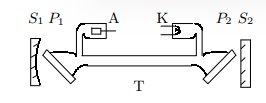
\includegraphics[width=5cm, height=3cm]{4.5.3-1}
	\caption{Устройство гелий-неонового лазера}
\end{wrapfigure}	 

\par \textbf{Устройство He-Ne лазера} Основным элементом Hе-Ne лазера непрерывного действия является газоразрядная трубка Т (рис. 1) с длиной несколько десятков сантиметров и с внутренним диаметром 5—10 мм. Трубка наполнена смесью гелия и неона с парциальными давлениями порядка 1 и 0,1 Торр соответственно. Концы трубки закрыты плоскопараллельными стеклянными или кварцевыми пластинами P1 и P2, установленными под углом Брюстера к ее оси. Линейно поляризованный свет с электрическим вектором, лежащим в плоскости падения, не испытывает потерь на
отражение, вследствие этого лазер генерирует линейно поляризованное излучение. В загнутых концах трубки располагаются анод А и катод К. Разряд в трубке возникает при напряжении 1,5–2 кВ. Трубка помещена между зеркалами S1 и S2, образующими интерферометр Фабри–Перо, который играет роль оптического резонатора. Прозрачность зеркал резонатора обычно меньше 1\%. Разрядный ток трубки составляет несколько десятков миллиампер.

\par Рабочим газом He-Ne-лазера является неон, ответственный за розовато-красное свечение разряда. Для возбуждения лазерной генерации необходимо создать инверсную заселенность уровней рабочего перехода неона. В гелий-неоновом лазере такая заселенность достигается главным образом из-за передачи возбуждения атомам неона от атомов гелия, которые возбуждаются в разряде электронным ударом.

\par Активная среда, обладающая инверсной заселенностью уровней, способна усиливать оптическое излучение на частоте рабочего перехода. Усиление происходит вследствие индуцированного (стимулированного) когерентного излучения возбужденных атомов под действием поля световой волны. Если кювету с активной средой поместить между зеркалами интерферометра Фабри–Перо, то испущенный вдоль
оси свет многократно отражается. При этом обеспечиваются условия возникновения лазерной генерации света. Условием возбуждения генерации является превышение усиления над потерями. Потери в Не-Neлазере обусловлены главным образом неидеальным отражением от зеркал (уход излучения из резонатора). Обратим в связи с этим еще раз внимание на установку пластин P1 и P2 (см. рис. 1) под углом Брюстера.

\par В интерферометрах Фабри–Перо, используемых в лазерах, излучение распространяется вдоль оси интерферометра. Если на полном оптическом пути 2L, где L — расстояние между зеркалами, укладывается целое число длин волн, наступает резонанс, т. е. в интерферометре возникает стоячая волна. При этом волна, дважды отраженная от зеркал, возвращается к испустившему ее атому в той же фазе, в которой она была испущена. Волны индуцированного излучения, складываясь, усиливают друг друга. Условие резонанса имеет вид

\begin{equation}
2L = m\lambda \text{(m - целое число)}
\end{equation}

\par Различным значениям порядка интерференции m соответствуют стоячие волны разных частот. Их называют типами колебаний, или модами. Из (1) легко получить выражение для межмодового расстояния $\Delta\nu$(в единицах частоты):

\begin{equation}
\Delta\nu = \frac{c}{2L} \;\;\;\;\;\;\;\;\;\; \text{(c - скорость света)}
\end{equation}

\par Из формулы (2) следует, что для интерферометра с базой L = 1 м межмодовое расстояние $\Delta\nu$ = 150 МГц. В то же время спектральная линия рабочего перехода неона имеет ширину порядка 1500 МГц. Генерация лазера возникает на резонансной частоте лазерного интерферометра. В нашем случае возможна одновременная генерация нескольких мод. Рисунок 2 иллюстрирует увеличение числа мод генерации лазера с ростом усиления активной среды, возникающим при увеличении мощности накачки. 

\begin{wrapfigure}[10]{r}{0.22\textheight}
	\vspace{-4ex}
	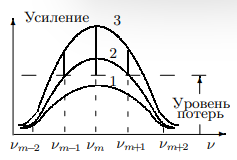
\includegraphics[width=6cm, height=3cm]{4.5.3-2}
	\caption{Развитие генерации лазера на нескольких модах при увеличении мощности накачки}
\end{wrapfigure}	 

\par Спектральная линия $\lambda$ = 632,8 нм неона уширена главным образом из-за эффекта Доплера, т. е. вследствие теплового движения атомов. При небольшом
усилении (кривая 1) генерации нет. В случае 2 генерация происходит только на частоте $\nu_m$, расположенной вблизи центра спектральной линии. Если усиление определяется кривой 3, генерация возникает на трех частотах: $\nu_{m-1}$, $\nu_{m}$ и $\nu_{m+1}$ и т. д. Говорят, что в этом случае лазер одновременно работает на трех модах.

\par Для гелий-неонового лазера с достаточно длинной трубкой на переходе 632,8 нм многомодовая генерация является обычным режимом работы

\par \textbf{Сканирующий интерферометр.} Для исследования межмодового состава излучения Не-Ne-лазера в работе используется сканирующий интерферометр, представляющий собой высокодобротный интерферометр Фабри–Перо с периодически изменяемой базой. Его
устройство схематически показано на рис. 3. 

\begin{wrapfigure}[9]{r}{0.18\textheight}
	\vspace{-4ex}
	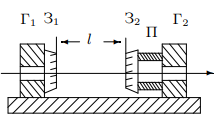
\includegraphics[width=5cm, height=2.5cm]{4.5.3-4}
	\caption{Устройство сканирующего интерферометра}
\end{wrapfigure}	 

\par Нa жестком массивном основании расположены две юстировочные головки Г1 и Г2, на которых укреплены зеркала З1 и З2. Зеркало
З1 установлено непосредственно на головке Г1, зеркало З2 связано с головкой Г2 через пьезокерамический элемент П. Юстировочные головки снабжены винтами (не показанными на рис. 3), которые
позволяют в небольших пределах поворачивать зеркала относительно вертикальной и горизонтальной осей. С помощью головок Г1 и Г2 зеркала выставляются на параллельность.

\par Пьезокерамический элемент П позволяет периодически изменять
базу интерферометра (l $\approx$ 10 см) на величину порядка длины световой волны. Элемент имеет форму полого цилиндра. Его внутренняя и наружная поверхности металлизированы и образуют цилиндрический конденсатор. Необходимое изменение длины цилиндра возникает при напряжении в несколько сот вольт. Если вдоль оси интерферометра распространяется световое излучение с длиной волны
$\lambda$, то при выполнении условия

\begin{equation}
2l = m\lambda \;\;\;\;\;\;\;\;\;\; \text{(m - целое число)}
\end{equation}

аналогичного условию (1) для лазера, возникает резонанс. Внешнее
излучение с длиной волны, удовлетворяющей условию (3), полностью
проходит через интерферометр. Если на интерферометр падает излучение с различными длинами волн, то одновременно может возникнуть несколько резонансов. Собственные моды интерферометра отличаются по частоте на величину

\begin{equation}
\Delta{f}=\frac{c}{2l}
\end{equation}

\par Величина $\Delta{f}$ называется дисперсионной областью спектрального прибора. В единицах $\lambda$ дисперсионная область сканирующего интерферометра равна

\begin{equation}
\Delta\lambda_{\text{СИ}} = \frac{\lambda}{m} = \frac{\lambda^2}{2l}
\end{equation}

\par В нашей работе интерферометр Фабри–Перо используется как спектральный прибор высокой разрешающей силы. Разрешающая способность R спектрального прибора определяется отношением

\begin{equation}
R = \frac{\lambda}{\delta\lambda}
\end{equation}

где $\delta\lambda$ — минимальная разность длин волн, разрешимая прибором вблизи длины волны $\lambda$. При определении $\delta\lambda$ обычно используют критерий разрешения Релея. Разрешающая способность интерферометра Фабри–Перо зависит от длины интерферометра l и коэффициента отражения зеркал r:

\begin{equation}
R = \frac{2\pi{l}}{\lambda(1-r)}
\end{equation}

В лазерной технике принято выражать разрешение интерферометра в единицах частоты:

\begin{equation}
\delta{f} = \nu\frac{\delta\lambda}{\lambda} = \frac{c}{2l}\frac{1-r}{\pi}
\end{equation}

\begin{wrapfigure}[14]{r}{0.18\textheight}
	\vspace{-4ex}
	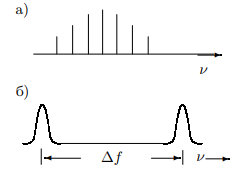
\includegraphics[width=5cm, height=4cm]{4.5.3-3}
	\caption{Спектр генерации лазера (а) и спектр пропускания сканирующего интерферометра (б)}
\end{wrapfigure}	 


\par Как видно из (8), величина $\frac{1-r}{\pi}$ показывает, во сколько раз разрешение интерферометра меньше его межмодового интервала. Сканирующий интерферометр, применяемый в настоящей работе, имеет зеркала с коэффициентом отражения r $\approx$ 98,5\%. Поэтому с его помощью можно разрешить две узкие спектральные линии, отличающиеся по частоте на величину порядка $0,005\delta{f}$, т. е. (при l = 10 см) приблизительно на 7,5 МГц. 

\par Рисунок 4 дает представление о соотношении между спектром генерации ОКГ и спектральной характеристикой сканирующего интерферометра (т. е. его спектром пропускания). Изменение расстояния между зеркалами сканирующего интерферометра приводит
к сдвигу нижней «гребенки» по оси частот. При этом интерферометр последовательно настраивается на разные моды лазера.

	\begin{figure}[h!]
		\begin{center}
			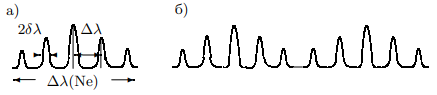
\includegraphics[width = 0.7\textwidth]{4.5.3-5}
			\caption{Характерные осциллограммы: амплитуда колебаний зеркала сканирующего интерферометра а) $\approx \Delta\lambda$(Ne); б) > 2$\Delta\lambda$(Ne)}
		\end{center}
	\end{figure}

\par Если одно из зеркал сканирующего интерферометра периодически
перемещать вдоль оси, мощность прошедшего через интерферометр излучения периодически изменяется (рис. 5).

\newpage
\subsection{Экспериментальная установка}

\begin{figure}[h!]
		\begin{center}
			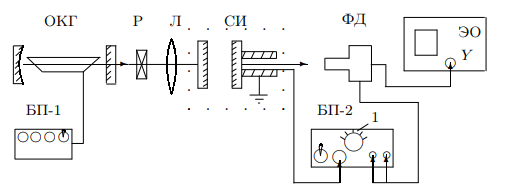
\includegraphics[width = 0.7\textwidth]{4.5.3-6}
			\caption{Схема установки для исследования доплеровского контура излучения лазера}
		\end{center}
	\end{figure}

\par Схема экспериментальной установки приведена на рис. 6. Излучение He-Ne лазера (ОКГ) проходит через поляризационную развязку Р и линзу Л и поступает на вход сканирующего интерферометра (СИ).

\par Поляризационная развязка предотвращает попадание в лазер излучения, отразившегося от элементов оптического тракта. Это излучение может существенно повлиять на работу лазера и даже привести к срыву генерации. Развязка состоит из поляроида и пластинки $\lambda$/4, главные направления которой установлены под углом $45^\circ$ по отношению к разрешённому направлению поляроида. После развязки Р свет приобретает циркулярную поляризацию (например, по правому кругу). При отражении от передней поверхности линзы, от зеркала сканирующего интерферометра и т. п. свет распространяется в обратном направлении в виде левополяризованной волны. Такая волна, пройдя через пластинку $\lambda$/4, вновь приобретает линейную поляризацию. Однако направление колебаний в этой волне оказывается перпендикулярным направлению разрешённых колебаний поляроида, так что до лазера волна не доходит.

\par Линза Л служит для формирования луча, поступающего на вход
сканирующего интерферометра. Линза снабжена поперечными и продольными салазками для юстировки прибора на максимум сигнала. С выхода сканирующего интерферометра излучение поступает на фотодиод ФД. Напряжение с фотодиода через усилитель подаётся на
вертикальный вход электронного осциллографа ЭО. ОКГ питается от блока питания БП-1, фотодиод и усилитель - от БП-2. Напряжение на пьезоэлемент сканирующего интерферометра подаётся с блока питания БП-2 и регулируется ручкой 1.

\newpage

\section{Результаты измерений и обработка данных}


\end{document}